\documentclass[journal]{IEEEtran}

\usepackage{amsmath,amssymb,amsfonts}
\usepackage{graphicx}
\usepackage{booktabs}
\usepackage{microtype}
\usepackage{url}
\usepackage{cite}
\usepackage{xcolor}
\usepackage{hyperref}

\hypersetup{
    colorlinks=true,
    linkcolor=blue,
    citecolor=blue,
    urlcolor=blue
}

\setlength{\textfloatsep}{4pt plus 1pt minus 1pt}
\setlength{\floatsep}{3pt plus 1pt minus 1pt}
\setlength{\dbltextfloatsep}{4pt plus 1pt minus 1pt}
\setlength{\dblfloatsep}{3pt plus 1pt minus 1pt}
\setlength{\intextsep}{4pt plus 1pt minus 1pt}
\setlength{\abovecaptionskip}{2pt plus 1pt minus 1pt}
\setlength{\belowcaptionskip}{1pt plus 1pt minus 1pt}
\renewcommand{\arraystretch}{0.92}

\begin{document}

\title{Supplementary Material: Physiology-Guided Temporal Fusion for Cross-Subject EEG--fNIRS Brain--Computer Interfaces}

\author{Hongjie~Chen and Fang~Duan%
\thanks{Hongjie Chen and Fang Duan are with the College of Information Science and Engineering, Huaqiao University, Xiamen 361021, China (e-mail: chenhj976@gmail.com; nkfetsh@gmail.com). Corresponding author: Fang Duan.}%
}

\markboth{IEEE Transactions on Biomedical Engineering,~Supplementary Material,~2026}%
{Chen and Duan: Supplementary Material}

\maketitle

\setcounter{table}{0}
\renewcommand{\thetable}{S\arabic{table}}
\setcounter{figure}{0}
\renewcommand{\thefigure}{S\arabic{figure}}

\section{Paradigm-Specific Neurovascular Dynamics: Mental Arithmetic vs.\ Motor Imagery}
\label{sec:supp_dynamics}

In this supplementary note, we provide empirical evidence and biophysical analysis regarding how neurovascular coupling (NVC) constraints operate across distinct functional regimes: metabolic-dominant cognitive processing (mental arithmetic, MA) versus rapid sensorimotor execution/imagery (motor imagery, MI).

\subsection{Neurovascular Divergence Between Cognitive and Sensorimotor Tasks}
Non-invasive electrophysiological (EEG) and hemodynamic (fNIRS) recordings capture fundamentally different physiological manifestations depending on cortical localization and task type:
\begin{enumerate}
    \item \textbf{Prefrontal Cognitive Processing (Mental Arithmetic):} Sustained arithmetic demands continuous executive control and working-memory retrieval in prefrontal cortex (PFC), electrophysiologically indexed by persistent frontal midline theta synchronization ($\theta$-ERS, 4--8\,Hz) \cite{gevins1997high}. Astrocytic end-feet sense synaptic glutamate release and initiate arteriole vasodilation, producing a delayed, highly concentrated hyperoxygenation response ($\Delta[\mathrm{HbO}]$ elevation and $\Delta[\mathrm{HbR}]$ washout) peaking at 4.5--6.5\,s \cite{attwell2010glial, iadecola2004neurovascular}. Consequently, the Gaussian latency kernel ($\tau_h \in [3.5, 6.5]$\,s) acts as a biophysical matched filter that captures this delayed metabolic surge while rejecting out-of-phase background fluctuations.
    \item \textbf{Sensorimotor Cortical Rhythms (Motor Imagery):} In contrast, motor imagery engages the primary motor and premotor cortices (M1/SMA) and is characterized by rapid event-related desynchronization (ERD) of $\mu$ (8--12\,Hz) and $\beta$ (13--30\,Hz) rhythms \cite{pfurtscheller1999event, mcfarland2000mu}. Although localized oxygen consumption occurs, sensorimotor vascular responses exhibit broader temporal dispersion and variable hemodynamic latencies across participants. Moreover, the primary discriminant information is rapidly decoded from the early electrophysiological desynchronization dynamics.
\end{enumerate}

\begin{figure*}[!t]
\centering
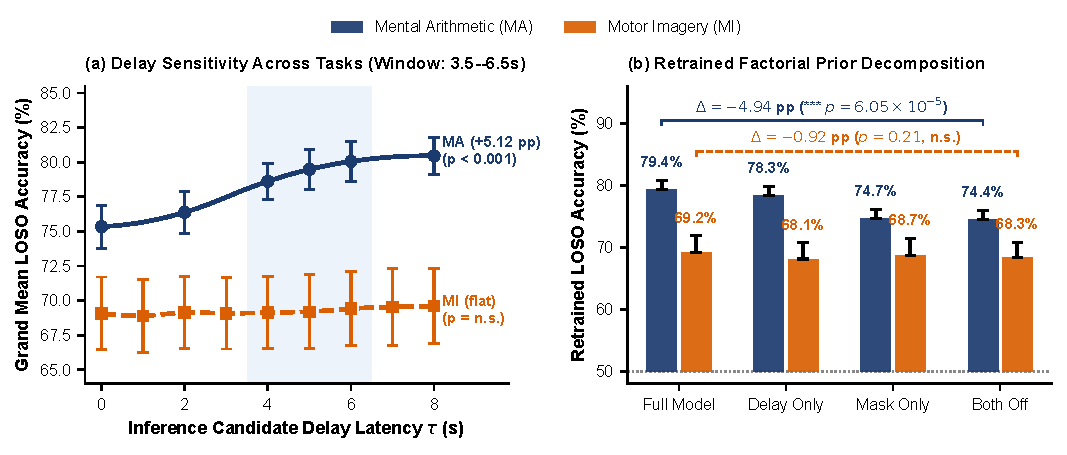
\includegraphics[width=0.84\textwidth]{figures/supplementary_fig_s1_delay_curves.pdf}
\caption{Cross-paradigm contrast of neurovascular temporal constraints across 29 held-out participants under leave-one-subject-out (LOSO) cross-validation. \textbf{(a)} Candidate delay sensitivity sweep ($\tau \in [0.0, 8.0]$\,s) evaluated on fixed-weight models: Mental arithmetic (MA, dark blue) displays strong delay resonance where accuracies peak within the canonical physiological window ($\ge 5.0$\,s, reaching 80.46\% at 8.0\,s, $+5.12$\,pp over $\tau=0$\,s, $p < 0.001$), whereas motor imagery (MI, orange dashed) exhibits delay invariance ($\le 0.69$\,pp variation across the entire 8\,s span). \textbf{(b)} $2 \times 2$ factorial prior retraining ablation ($P$: Gaussian delay prior, $M$: physical causal mask): MA demonstrates a statistically significant drop of $-4.94$\,pp ($p = 6.05 \times 10^{-5}$) upon unconstrained attention ($P_{\mathrm{off}}, M_{\mathrm{off}}$), while MI displays negligible sensitivity ($-0.92$\,pp, $p = 0.2128$, not statistically significant).}
\label{fig:supp_s1}
\end{figure*}

\subsection{Empirical Validation via Candidate Delay Sweeps and Factorial Retraining}
To evaluate these biophysical dynamics, we conducted two controlled investigations across all 29 participants of the Shin et al.\ (2017) Motor Imagery dataset \cite{shin2017open} (1,740 trials, left vs.\ right hand MI) and compared them with the TU Berlin Mental Arithmetic benchmark \cite{shin2017open}:
\begin{itemize}
    \item \textbf{Experiment 1 (Delay Sensitivity):} Inference delays $\tau \in \{0.0, 1.0, 2.0, 3.0, 4.0, 5.0, 6.0, 7.0, 8.0\}$\,s were evaluated on fixed models (Fig.~\ref{fig:supp_s1}a). On MA, accuracy is sharply dependent on $\tau$, increasing from 75.34\% ($\tau=0$\,s) to 80.46\% ($\tau=8.0$\,s, $+5.12$\,pp, $p < 0.001$). On MI, accuracy remains flat across the entire 8-second range (68.91\% to 69.60\%, $\Delta_{\max} = 0.69$\,pp, $p = \mathrm{n.s.}$).
    \item \textbf{Experiment 2 ($2 \times 2$ Factorial Prior Retraining):} Retrained models from scratch across all 29 LOSO folds under four orthogonal prior configurations: (i) Full Model ($P_{\mathrm{on}}, M_{\mathrm{on}}$), (ii) Delay Only ($P_{\mathrm{on}}, M_{\mathrm{off}}$), (iii) Mask Only ($P_{\mathrm{off}}, M_{\mathrm{on}}$), and (iv) Both Priors Off ($P_{\mathrm{off}}, M_{\mathrm{off}}$, unconstrained attention). As depicted in Fig.~\ref{fig:supp_s1}b, removing temporal priors on MA degrades accuracy by $-4.94$\,pp ($p = 6.05 \times 10^{-5}$), confirming that unconstrained attention overfits spurious cross-subject correlations. On MI, removing both priors produces only a $-0.92$\,pp change ($p = 0.2128$), demonstrating that sensorimotor decoding relies less on strict hemodynamic phase alignment.
\end{itemize}

\begin{table*}[!t]
\centering
\caption{Comprehensive Numerical Performance Breakdown across 29 LOSO Folds: Mental Arithmetic (MA) vs.\ Motor Imagery (MI)}
\label{tab:supp_s1}
{\scriptsize
\setlength{\tabcolsep}{4.2pt}
\begin{tabular}{lcccccc}
\toprule
& \multicolumn{3}{c}{\textbf{Mental Arithmetic (Shin et al.\ 2017)}} & \multicolumn{3}{c}{\textbf{Motor Imagery (Shin et al.\ 2017)}} \\
\cmidrule(lr){2-4} \cmidrule(lr){5-7}
Experimental Condition / Factor & Accuracy (\%) & Macro F1 (\%) & 95\% Conf.\ Int.\ (\%) & Accuracy (\%) & Macro F1 (\%) & 95\% Conf.\ Int.\ (\%) \\
\midrule
\multicolumn{7}{l}{\textit{\textbf{Part A: Fixed-Weight Candidate Delay Latency Sweep ($\tau \in [0.0, 8.0]$\,s)}}} \\
\quad $\tau = 0.0$\,s (Zero Latency Shift) & 75.34 $\pm$ 8.35 & 74.96 $\pm$ 8.44 & [72.17, 78.52] & 69.08 $\pm$ 14.14 & 66.82 $\pm$ 16.14 & [63.70, 74.46] \\
\quad $\tau = 1.0$\,s & --- & --- & --- & 68.91 $\pm$ 14.25 & 66.65 $\pm$ 16.21 & [63.49, 74.33] \\
\quad $\tau = 2.0$\,s & 76.38 $\pm$ 8.19 & 76.02 $\pm$ 8.28 & [73.26, 79.49] & 69.14 $\pm$ 13.95 & 66.90 $\pm$ 16.02 & [63.83, 74.44] \\
\quad $\tau = 3.0$\,s & --- & --- & --- & 69.08 $\pm$ 13.86 & 66.79 $\pm$ 15.98 & [63.81, 74.35] \\
\quad $\tau = 4.0$\,s & 78.62 $\pm$ 6.97 & 78.36 $\pm$ 7.09 & [75.97, 81.27] & 69.14 $\pm$ 14.08 & 66.92 $\pm$ 16.11 & [63.78, 74.50] \\
\quad $\tau = 5.0$\,s (Canonical Prior Mean) & 79.48 $\pm$ 7.75 & 79.28 $\pm$ 7.82 & [76.53, 82.43] & 69.20 $\pm$ 14.41 & 67.00 $\pm$ 16.41 & [63.71, 74.68] \\
\quad $\tau = 6.0$\,s & 80.06 $\pm$ 7.66 & 79.87 $\pm$ 7.74 & [77.14, 82.97] & 69.43 $\pm$ 14.53 & 67.24 $\pm$ 16.50 & [63.90, 74.96] \\
\quad $\tau = 7.0$\,s & --- & --- & --- & 69.54 $\pm$ 14.89 & 67.35 $\pm$ 16.82 & [63.88, 75.20] \\
\quad $\tau = 8.0$\,s & \textbf{80.46 $\pm$ 7.11} & \textbf{80.31 $\pm$ 7.20} & [77.75, 83.16] & \textbf{69.60 $\pm$ 14.52} & \textbf{67.41 $\pm$ 16.53} & [64.07, 75.12] \\
\midrule
\multicolumn{7}{l}{\textit{\textbf{Part B: $2 \times 2$ Factorial Prior Retraining Ablation across 29 Folds}}} \\
\quad Full Model ($P_{\mathrm{on}}, M_{\mathrm{on}}$) & \textbf{79.37 $\pm$ 7.73} & \textbf{79.15 $\pm$ 7.82} & [76.43, 82.31] & \textbf{69.20 $\pm$ 14.40} & \textbf{67.00 $\pm$ 16.41} & [63.71, 74.68] \\
\quad Delay Prior Only ($P_{\mathrm{on}}, M_{\mathrm{off}}$) & 78.33 $\pm$ 8.07 & 78.11 $\pm$ 8.12 & [75.26, 81.40] & 68.10 $\pm$ 14.03 & 65.79 $\pm$ 16.27 & [62.77, 73.44] \\
\quad Causal Mask Only ($P_{\mathrm{off}}, M_{\mathrm{on}}$) & 74.66 $\pm$ 7.96 & 74.38 $\pm$ 8.01 & [71.63, 77.68] & 68.68 $\pm$ 14.85 & 66.26 $\pm$ 17.34 & [63.03, 74.32] \\
\quad Both Priors Off ($P_{\mathrm{off}}, M_{\mathrm{off}}$) & 74.43 $\pm$ 8.34 & 74.08 $\pm$ 8.41 & [71.26, 77.60] & 68.28 $\pm$ 13.72 & 66.06 $\pm$ 15.80 & [63.06, 73.49] \\
\bottomrule
\end{tabular}}
\par\vspace{1pt}
{\scriptsize Evaluated under 29-fold LOSO cross-validation with unsupervised Euclidean Alignment (EA) applied individually per participant. Part A tests fixed-weight delay sensitivity across candidate $\tau$ latencies. Part B retrains each model variant from scratch under identical hyperparameter conditions across all 29 folds. For MA, removing both priors yields $\Delta = -4.94$\,pp ($p = 6.05 \times 10^{-5}$, Wilcoxon signed-rank test). For MI, removing both priors yields $\Delta = -0.92$\,pp ($p = 0.2128$, n.s.).}
\end{table*}

\section{Methodological Specifications of the Motor Imagery Investigation}
\label{sec:supp_methods}

To guarantee full reproducibility, the implementation protocol for the Motor Imagery investigation is detailed as follows:
\begin{enumerate}
    \item \textbf{Dataset Details:} The cohort comprises 29 healthy adults performing 30 trials of left-hand and 30 trials of right-hand motor imagery (60 trials per participant, 1,740 trials total) recorded by Shin et al.\ (2017) \cite{shin2017open}.
    \item \textbf{Electrophysiological Preprocessing:} 30 scalp EEG channels covering frontal, central, and parietal regions were bandpass filtered between 0.5 and 40\,Hz. Unsupervised Euclidean Alignment (EA) \cite{he2019transfer} was computed on each participant's covariance matrix $\bar{R} = \frac{1}{N} \sum_{i=1}^N X_i X_i^T + 10^{-5} I$ to eliminate inter-subject covariance drift without label supervision.
    \item \textbf{Hemodynamic Preprocessing:} 72 fNIRS channels (36 $\Delta[\mathrm{HbO}]$, 36 $\Delta[\mathrm{HbR}]$) sampled at 10.33\,Hz were bandpass filtered (0.01--0.10\,Hz) via zero-phase 4th-order Butterworth filters to eliminate cardiac and respiratory rhythms.
    \item \textbf{Participant-Isolated LOSO Protocol:} Each fold isolates one participant as the held-out test subject. Among the remaining 28 participants, 23 participants are allocated for training and 5 participants are reserved for validation (checkpoint selection). Hyperparameters strictly mirror the main benchmark: AdamW optimizer, learning rate $3 \times 10^{-3}$, weight decay 0.05, batch size 128, and 15 epochs with warmup cosine scheduling.
\end{enumerate}

\section{Conclusion}
These supplementary findings validate that while unconstrained cross-modal attention is capable of capturing immediate sensorimotor interactions, biophysical latency priors provide decisive inductive bias in metabolically driven cognitive regimes, enabling zero-calibration cross-subject generalizability.

{\footnotesize
\begin{thebibliography}{10}\setlength{\itemsep}{0pt}\setlength{\parskip}{0pt}
\bibitem{gevins1997high}
A.~Gevins, M.~E. Smith, L.~McEvoy, and D.~Yu, ``High-resolution EEG mapping of cortical activation related to working memory: effects of task difficulty, type of processing, and practice,'' \textit{Cerebral Cortex}, vol.~7, no.~4, pp.~374--385, 1997.

\bibitem{attwell2010glial}
D.~Attwell, A.~M. Buchan, S.~Charpak, M.~Lauritzen, B.~A. MacVicar, and E.~A. Newman, ``Glial and neuronal control of brain blood flow,'' \textit{Nature}, vol.~468, no.~7321, pp.~232--243, 2010.

\bibitem{iadecola2004neurovascular}
C.~Iadecola, ``Neurovascular regulation in the normal brain and in Alzheimer's disease,'' \textit{Nature Reviews Neuroscience}, vol.~5, no.~5, pp.~347--360, 2004.

\bibitem{pfurtscheller1999event}
G.~Pfurtscheller and F.~H. Lopes~da~Silva, ``Event-related EEG/MEG synchronization and desynchronization: basic principles,'' \textit{Clinical Neurophysiology}, vol.~110, no.~11, pp.~1842--1857, 1999.

\bibitem{mcfarland2000mu}
D.~J. McFarland, L.~A. Miner, T.~M. Vaughan, and J.~R. Wolpaw, ``Mu and beta rhythm topographies during motor imagery and actual movements,'' \textit{Brain Topography}, vol.~12, no.~3, pp.~177--186, 2000.

\bibitem{shin2017open}
J.~Shin, K.-R. M{\"u}ller, and F.~B. Hwang, ``An open dataset for EEG and fNIRS-based BCI with visual and arithmetic tasks,'' \textit{Frontiers in Human Neuroscience}, vol.~11, p.~109, 2017.

\bibitem{he2019transfer}
H.~He and D.~Wu, ``Transfer learning for brain--computer interfaces: A Euclidean space data alignment approach,'' \textit{IEEE Transactions on Biomedical Engineering}, vol.~67, no.~2, pp.~399--410, 2020.
\end{thebibliography}
}

\end{document}
